\documentclass{beamer}
\usepackage[utf8]{inputenc}
\usepackage{graphicx, epsfig}
\usepackage{amsmath,mathrsfs,amsfonts,amssymb}
%\usepackage{subfig}
\usepackage{floatflt}
\usepackage{epic,ecltree}
\usepackage{mathtext}
\usepackage{fancybox}
\usepackage{fancyhdr}
\usepackage{multirow}
\usepackage{enumerate}
\usepackage{epstopdf}
\usepackage{multicol}
\usepackage{algorithm}
\usepackage[noend]{algorithmic}
\usepackage{tikz}
\usepackage{blindtext}
\usetheme{default}%{Singapore}%{Warsaw}%{Warsaw}%{Darmstadt}
\usecolortheme{default}
\setbeamerfont{title}{size=\Huge}
\setbeamertemplate{footline}[page number]{}


\makeatletter
\newcommand\HUGE{\@setfontsize\Huge{35}{40}}
\makeatother    

\setbeamerfont{title}{size=\HUGE}
\beamertemplatenavigationsymbolsempty

% latin bold lower
\newcommand{\ba}{\mathbf{a}} 
\newcommand{\bc}{\mathbf{c}} 
\newcommand{\be}{\mathbf{e}} 
\newcommand{\bh}{\mathbf{h}} 
\newcommand{\bp}{\mathbf{p}} 
\newcommand{\bt}{\mathbf{t}} 
\newcommand{\bs}{\mathbf{s}} 
\newcommand{\bu}{\mathbf{u}} 
\newcommand{\bv}{\mathbf{v}} 
\newcommand{\bw}{\mathbf{w}} 
\newcommand{\bx}{\mathbf{x}} 
\newcommand{\by}{\mathbf{y}} 
\newcommand{\bz}{\mathbf{z}} 

% latin bold upper
\newcommand{\bA}{\mathbf{A}} 
\newcommand{\bB}{\mathbf{B}} 
\newcommand{\bC}{\mathbf{C}} 
\newcommand{\bI}{\mathbf{I}} 
\newcommand{\bL}{\mathbf{L}} 
\newcommand{\bM}{\mathbf{M}} 
\newcommand{\bQ}{\mathbf{Q}} 
\newcommand{\bT}{\mathbf{T}} 
\newcommand{\bU}{\mathbf{U}} 
\newcommand{\bV}{\mathbf{V}} 
\newcommand{\bW}{\mathbf{W}} 
\newcommand{\bX}{\mathbf{X}} 
\newcommand{\bY}{\mathbf{Y}} 
\newcommand{\bZ}{\mathbf{Z}} 

% latin cal upper
\newcommand{\cG}{\mathcal{G}} 
\newcommand{\cL}{\mathcal{L}} 
\newcommand{\cN}{\mathcal{N}} 
\newcommand{\cS}{\mathcal{S}} 
\newcommand{\cT}{\mathcal{T}} 
\newcommand{\cW}{\mathcal{W}} 
\newcommand{\cX}{\mathcal{X}} 
\newcommand{\cZ}{\mathcal{Z}} 

% latin bb upper
\newcommand{\bbE}{\mathbb{E}} 
\newcommand{\bbI}{\mathbb{I}} 
\newcommand{\bbP}{\mathbb{P}} 
\newcommand{\bbR}{\mathbb{R}} 

% greek bold lower
\newcommand{\bepsilon}{\boldsymbol{\epsilon}} 
\newcommand{\btheta}{\boldsymbol{\theta}} 
\newcommand{\blambda}{\boldsymbol{\lambda}} 
\newcommand{\bpi}{\boldsymbol{\pi}} 
\newcommand{\bmu}{\boldsymbol{\mu}} 
\newcommand{\bsigma}{\boldsymbol{\sigma}} 
\newcommand{\bphi}{\boldsymbol{\phi}} 

% greek bold upper
\newcommand{\bSigma}{\boldsymbol{\Sigma}} 

\DeclareMathOperator*{\argmin}{arg\,min}
\DeclareMathOperator*{\argmax}{arg\,max}

\newcommand{\createdgmtitle}[1]{\title[\hbox to 56mm{Deep Generative Models  \hfill\insertframenumber\,/\,\inserttotalframenumber}]
	{\vspace{1.5cm} \\ Deep Generative Models \\ {\Huge Lecture #1}}
	\author{Roman Isachenko}
	\institute{
	Moscow Institute of Physics and Technology
	} 
	\date{Autumn, 2021}
}

\newcommand\myfootnote[1]{%
  \tikz[remember picture,overlay]
  \draw (current page.south west) +(1in + \oddsidemargin,0.5em)
  node[anchor=south west,inner sep=0pt]{\parbox{\textwidth}{%
      \rlap{\rule{10em}{0.4pt}}\raggedright\scriptsize \textit{#1}}};}

\newcommand\myfootnotewithlink[2]{%
  \tikz[remember picture,overlay]
  \draw (current page.south west) +(1in + \oddsidemargin,0.5em)
  node[anchor=south west,inner sep=0pt]{\parbox{\textwidth}{%
      \rlap{\rule{10em}{0.4pt}}\raggedright\scriptsize\href{#1}{\textit{#2}}}};}
\createdgmtitle{4}
%--------------------------------------------------------------------------------
\begin{document}
%--------------------------------------------------------------------------------
\begin{frame}[noframenumbering,plain]
%\thispagestyle{empty}
\titlepage
\end{frame}
%======
\begin{frame}{Recap of previous lecture}
	\begin{block}{Latent variable models (LVM)}
		\vspace{-0.3cm}
		\[
			p(\bx | \btheta) = \int p(\bx, \bz | \btheta) d\bz = \int p(\bx | \bz, \btheta) p(\bz) d\bz.
		\]
	\end{block}
	\begin{block}{MLE problem for LVM}
		\vspace{-0.7cm}
		\begin{multline*}
			\btheta^* = \argmax_{\btheta} \log p(\bX| \btheta) = \argmax_{\btheta} \sum_{i=1}^n \log p(\bx_i | \btheta) = \\ = \argmax_{\btheta} \log \sum_{i=1}^n \int p(\bx_i| \bz_i, \btheta) p(\bz_i) d\bz_i.
		\end{multline*}
		\vspace{-0.7cm}
	\end{block}
	\begin{block}{Naive Monte-Carlo estimation}
		\vspace{-0.7cm}
		\[
			p(\bx | \btheta) = \int p(\bx | \bz, \btheta) p(\bz) d\bz = \bbE_{p(\bz)} p(\bx | \bz, \btheta) \approx \frac{1}{K} \sum_{k=1}^{K} p(\bx | \bz_k, \btheta),
		\]
		\vspace{-0.5cm} \\
		where $\bz_k \sim p(\bz)$. 
	\end{block}
\end{frame}
%======
\begin{frame}{Recap of previous lecture}
	\begin{block}{Variational lower Bound (ELBO)}
		\vspace{-0.3cm}
		\[
			\log p(\bx| \btheta) = \mathcal{L} (q, \btheta) + KL(q(\bz) || p(\bz|\bx, \btheta)) \geq \mathcal{L} (q, \btheta).
		\]
	\end{block}
	
	\vspace{-0.5cm}
	\[
	 \mathcal{L} (q, \btheta) = \int q(\bz) \log \frac{p(\bx, \bz | \btheta)}{q(\bz)}d\bz = \mathbb{E}_{q} \log p(\bx | \bz, \btheta) - KL (q(\bz) || p(\bz))
	\]
	\vspace{-0.3cm}
	\begin{block}{Log-likelihood decomposition}
		\vspace{-0.5cm}
		\[
		 \log p(\bx| \btheta) = \mathbb{E}_{q} \log p(\bx | \bz, \btheta) - KL (q(\bz) || p(\bz)) + KL(q(\bz) || p(\bz|\bx, \btheta)).
		\]
	\end{block}
	\begin{itemize}
	\item Instead of maximizing incomplete likelihood, maximize ELBO
   	\[
  \max_{\btheta} p(\bx | \btheta) \quad \rightarrow \quad \max_{q, \btheta} \mathcal{L} (q, \btheta)
   	\]
   	\item Maximization of ELBO by variational distribution $q$ is equivalent to minimization of KL
  	\[
  \max_q \mathcal{L} (q, \btheta) \equiv \min_q KL(q(\bz) || p(\bz|\bx, \btheta)).
  	\]
  	\end{itemize}
		   	    
\end{frame}

\begin{frame}{Recap of previous lecture}
	\begin{block}{EM-algorithm}
	\begin{itemize}
		\item E-step
		\[
			q^*(\bz) = \argmax_q \mathcal{L} (q, \btheta^*)
			= \argmin_q KL(q(\bz) || p(\bz | \bx, \btheta^*));
		\]
		\item M-step
		\[
			\btheta^* = \argmax_{\btheta} \mathcal{L} (q^*, \btheta);
		\]
	\end{itemize}
	\vspace{-0.3cm}
	\end{block}
	\begin{block}{Amortized variational inference}
	Restrict a family of all possible distributions $q(\bz)$ to a parametric class $q(\bz|\bx, \bphi)$ conditioned on samples $\bx$ with parameters $\bphi$.
	\end{block}
	
	\textbf{Variational Bayes}
	\begin{itemize}
		\item E-step
		\[
		\bphi_k = \bphi_{k-1} + \left.\eta \nabla_{\bphi} \mathcal{L}(\bphi, \btheta_{k-1})\right|_{\bphi=\bphi_{k-1}}
		\]
		\item M-step
		\[
		\btheta_k = \btheta_{k-1} + \left.\eta \nabla_{\btheta} \mathcal{L}(\bphi_k, \btheta)\right|_{\btheta=\btheta_{k-1}}
		\]
	\end{itemize}
\end{frame}
%=======
\begin{frame}{ELBO gradients}
	\[
		 \mathcal{L} (\bphi, \btheta)  = \mathbb{E}_{q} \left[\log p(\bx | \bz, \btheta) + \log \frac{p(\bz)}{q(\bz | \bx, \bphi)} \right] \rightarrow \max_{\bphi, \btheta}.
	\]	
	\begin{block}{M-step: $\nabla_{\btheta} \mathcal{L}(\bphi, \btheta)$}
		\vspace{-0.7cm}
		\begin{multline*}
			\nabla_{\btheta} \mathcal{L} (\bphi, \btheta)
			= \int q(\bz|\bx, \bphi) \nabla_{\btheta}\log p(\bx|\bz, \btheta) d \bz \approx  \\
			\approx \nabla_{\btheta}\log p(\bx|\bz^*, \btheta), \quad \bz^* \sim q(\bz|\bx, \bphi).
		\end{multline*}
		\vspace{-0.7cm}
	\end{block}
	\begin{block}{E-step: $\nabla_{\bphi} \mathcal{L}(\bphi, \btheta)$}
	Difference from M-step: density function $q(\bz| \bx, \bphi)$ depends on the parameters $\bphi$, it is impossible to use the Monte-Carlo estimation:
	\begin{align*}
		\nabla_{\bphi} \mathcal{L} (\bphi, \btheta) &= \nabla_{\bphi} \int q(\bz | \bx, \bphi) \left[\log p(\bx | \bz, \btheta) + \log \frac{p(\bz)}{q(\bz| \bx, \bphi)} \right] d \bz \\
		& \neq  \int q(\bz | \bx, \bphi) \nabla_{\bphi} \left[\log p(\bx | \bz, \btheta) + \log \frac{p(\bz)}{q(\bz| \bx, \bphi)} \right] d \bz \\
	\end{align*}
	\end{block}
\end{frame}
%======
\begin{frame}{Reparametrization trick}
	\begin{block}{Law of the unconscious statistician (LOTUS)}
		Let $X$ be a random variable and let $Y=g(X)$. Then
		\[
			\bbE_{p_Y} Y = \bbE_{p_X} g(X) = \int g(\bx) p(\bx) d \bx.
		\]
		\vspace{-0.3cm}
	\end{block}
	\begin{block}{Examples} 
		\begin{itemize}
		\item $r(x) = \mathcal{N}(x|0, 1)$, $y = \sigma \cdot x + \mu$, $p_Y(y|\theta) = \mathcal{N}(y| \mu, \sigma^2)$, $\theta = [\mu, \sigma]$.

		\item $\bepsilon^* \sim r(\bepsilon), \quad \bz = g(\bx, \bepsilon, \bphi), \quad \bz \sim q(\bz | \bx, \bphi)$
		\begin{multline*}
			\nabla_{\bphi}\int q(\bz|\bx, \bphi) f(\bz) d\bz = \nabla_{\bphi}\int r(\bepsilon)  f(\bz) d\bepsilon \\ = \int r(\bepsilon) \nabla_{\bphi} f(g(\bx, \bepsilon, \bphi)) d\bepsilon \approx \nabla_{\bphi} f(g(\bx, \bepsilon^*, \bphi))
		\end{multline*}
		\end{itemize}
	\end{block}
\end{frame}
%=======
\begin{frame}{ELBO gradient (E-step, $\nabla_{\bphi} \mathcal{L}(\bphi, \btheta)$)}
	\vspace{-0.5cm}
	\begin{multline*}
		\nabla_{\bphi} \mathcal{L} (\bphi, \btheta) = \nabla_{\bphi}\int q(\bz|\bx, \bphi) \log p(\bx| \bz, \btheta)  d\bz - \nabla_{\bphi} \text{KL}(q(\bz | \bx, \bphi) || p(\bz))
		\\ = \int r(\bepsilon) \nabla_{\bphi} \log p(\bx | g(\bx, \bepsilon, \bphi), \btheta) d\bepsilon  - \nabla_{\bphi} \text{KL}(q(\bz | \bx, \bphi) || p(\bz))
		\\ \approx \nabla_{\bphi} \log p(\bx | g(\bx, \bepsilon^*, \bphi), \btheta)  - \nabla_{\bphi} \text{KL}(q(\bz | \bx, \bphi) || p(\bz))
	\end{multline*}
	\vspace{-0.5cm}
	\begin{block}{Variational assumption}
		\vspace{-0.3cm}
		\[
			r(\bepsilon) = \mathcal{N}(0, \bI); \quad  q(\bz| \bx, \bphi) = \mathcal{N} (\bmu_{\bphi}(\bx), \bsigma^2_{\bphi}(\bx)).
		\]
		\[
			\bz = g(\bx, \bepsilon, \bphi) = \bsigma_{\bphi}(\bx) \cdot \bepsilon + \bmu_{\bphi}(\bx).
		\]
		Here $\bmu_{\bphi}(\cdot), \bsigma_{\bphi}(\cdot)$ are parameterized functions (outputs of neural network).
	\end{block}
	\begin{itemize}
		\item $p(\bz)$ -- prior distribution on latent variables $\bz$. We could specify any distribution that we want. Let say $p(\bz) = \cN (0, \bI)$.
		\item $p(\bx | \bz, \btheta)$ - generative distibution. Since it is a parameterized function let it be neural network with parameters $\btheta$.
	\end{itemize}
\end{frame}
%=======
\begin{frame}{Variational autoencoder (VAE)}
	\begin{block}{Final algorithm}
		\begin{itemize}
			\item pick random sample $\bx_i, i \sim U[1, n]$.
			\item compute the objective:
			\vspace{-0.3cm}
			\[
				\bepsilon^* \sim r(\bepsilon); \quad \bz^* = g(\bx, \bepsilon^*, \bphi);
			\]
			\[
				\cL(\bphi, \btheta) \approx  \log p(\bx | \bz^*, \btheta) - KL(q(\bz^* | \bx, \bphi) || p(\bz^*)).
			\]
			\item compute a stochastic gradients w.r.t. $\bphi$ and $\btheta$
			\begin{align*}
				\nabla_{\bphi} \mathcal{L} (\bphi, \btheta) &\approx \nabla_{\bphi} \log p(\bx | g(\bx, \bepsilon^*, \bphi), \btheta)  - \nabla_{\bphi} \text{KL}(q(\bz | \bx, \bphi) || p(\bz)); \\
				\nabla_{\btheta} \mathcal{L} (\bphi, \btheta) &\approx \nabla_{\btheta} \log p(\bx|\bz^*, \btheta).
			\end{align*}
			\item update $\btheta, \bphi$ according to the selected optimization method (SGD, Adam, RMSProp):
			\begin{align*}
				\bphi &:= \bphi + \eta \nabla_{\bphi} \mathcal{L}(\bphi, \btheta), \\
				\btheta &:= \btheta + \eta \nabla_{\btheta} \mathcal{L}(\bphi, \btheta).
			\end{align*}
		\end{itemize}
	\end{block}
\end{frame}
%=======
\begin{frame}{Variational autoencoder (VAE)}
	\begin{minipage}[t]{0.55\columnwidth}
	    \begin{itemize}
	    \item VAE learns stochastic mapping between $\bx$-space, from complicated distribution $\pi(\bx)$, and a latent $\bz$-space, with simple distribution. 
	    \item The generative model learns a joint distribution $p(\bx, \bz | \btheta) = p(\bz) p(\bx |\bz, \btheta)$, with a prior distribution $p(\bz)$, and a stochastic decoder $p(\bx|\bz, \btheta)$. 
	    \item The stochastic encoder $q(\bz|\bx, \bphi)$ (inference model), approximates the true but intractable posterior $p(\bz|\bx, \btheta)$ of the generative model.
	    \end{itemize}
	\end{minipage}%
	\begin{minipage}[t]{0.45\columnwidth}
		\begin{figure}[h]
			\centering
			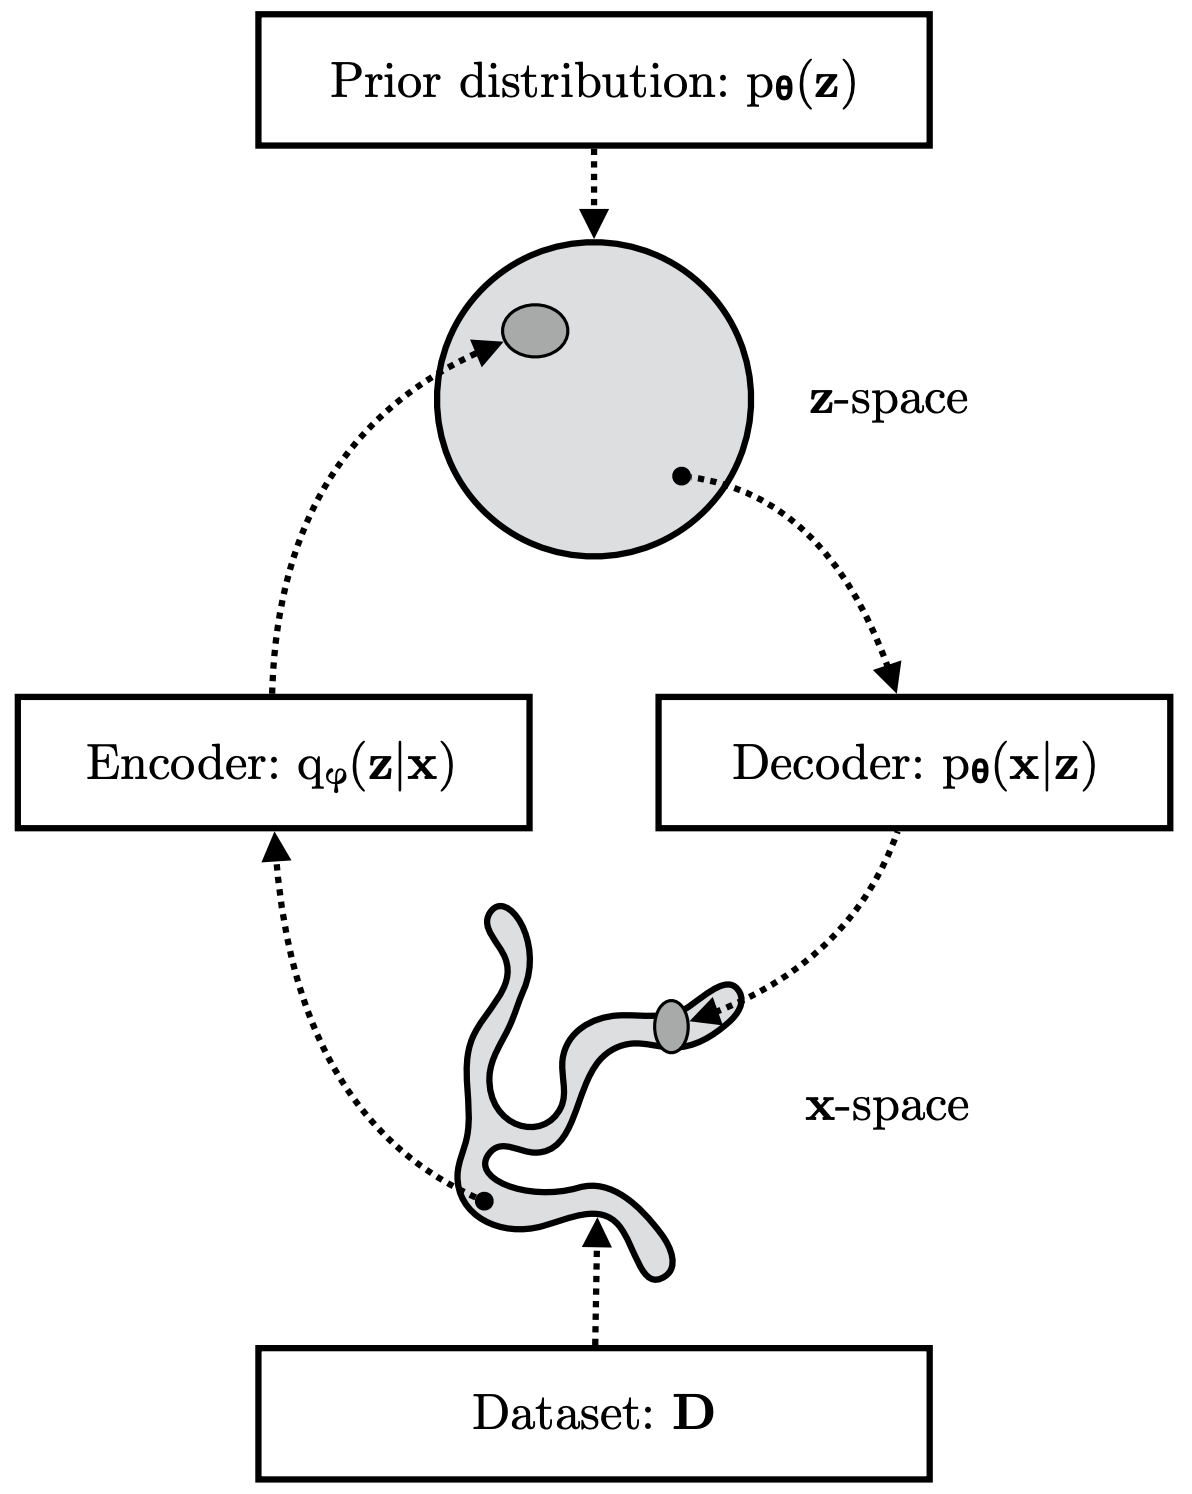
\includegraphics[width=\linewidth]{figs/vae_scheme}
		\end{figure}
	\end{minipage}
	
	\myfootnotewithlink{https://arxiv.org/abs/1906.02691}{Kingma D. P., Welling M. An introduction to variational autoencoders, 2019}
\end{frame}
%=======
\begin{frame}{Variational Autoencoder}
	\begin{figure}[h]
		\centering
		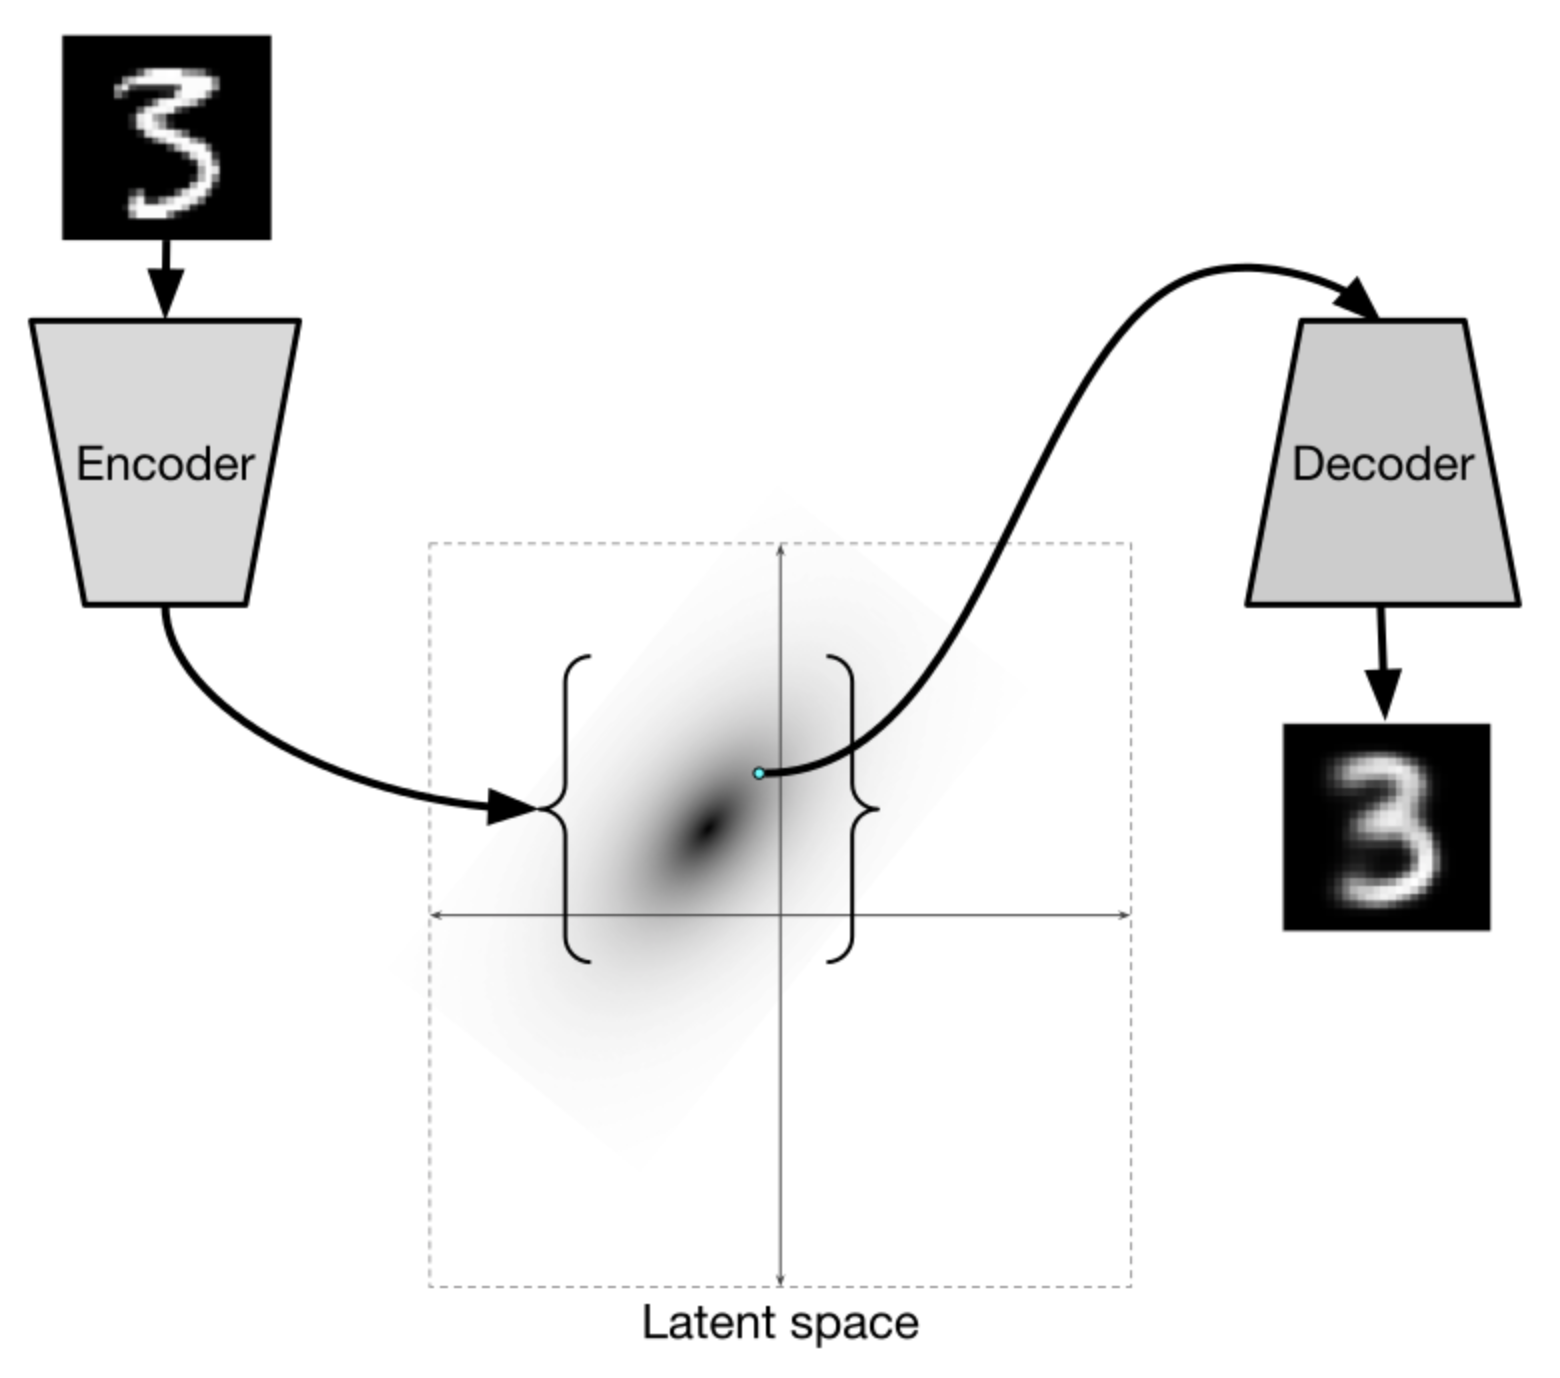
\includegraphics[width=.7\linewidth]{figs/VAE.png}
	\end{figure}
	\myfootnotewithlink{http://ijdykeman.github.io/ml/2016/12/21/cvae.html}{image credit: http://ijdykeman.github.io/ml/2016/12/21/cvae.html}
\end{frame}
%=======
\begin{frame}{Variational autoencoder (VAE)}
	\begin{itemize}
		\item Encoder $q(\bz | \bx, \bphi) = \text{NN}_e(\bx, \bphi)$ outputs $\bmu_{\bphi}(\bx)$ and $\bsigma_{\bphi}(\bx)$.
		\item Decoder $p(\bx | \bz, \btheta) = \text{NN}_d(\bz, \btheta)$ outputs parameters of the sample distribution.
	\end{itemize}
	\begin{figure}[h]
		\centering
		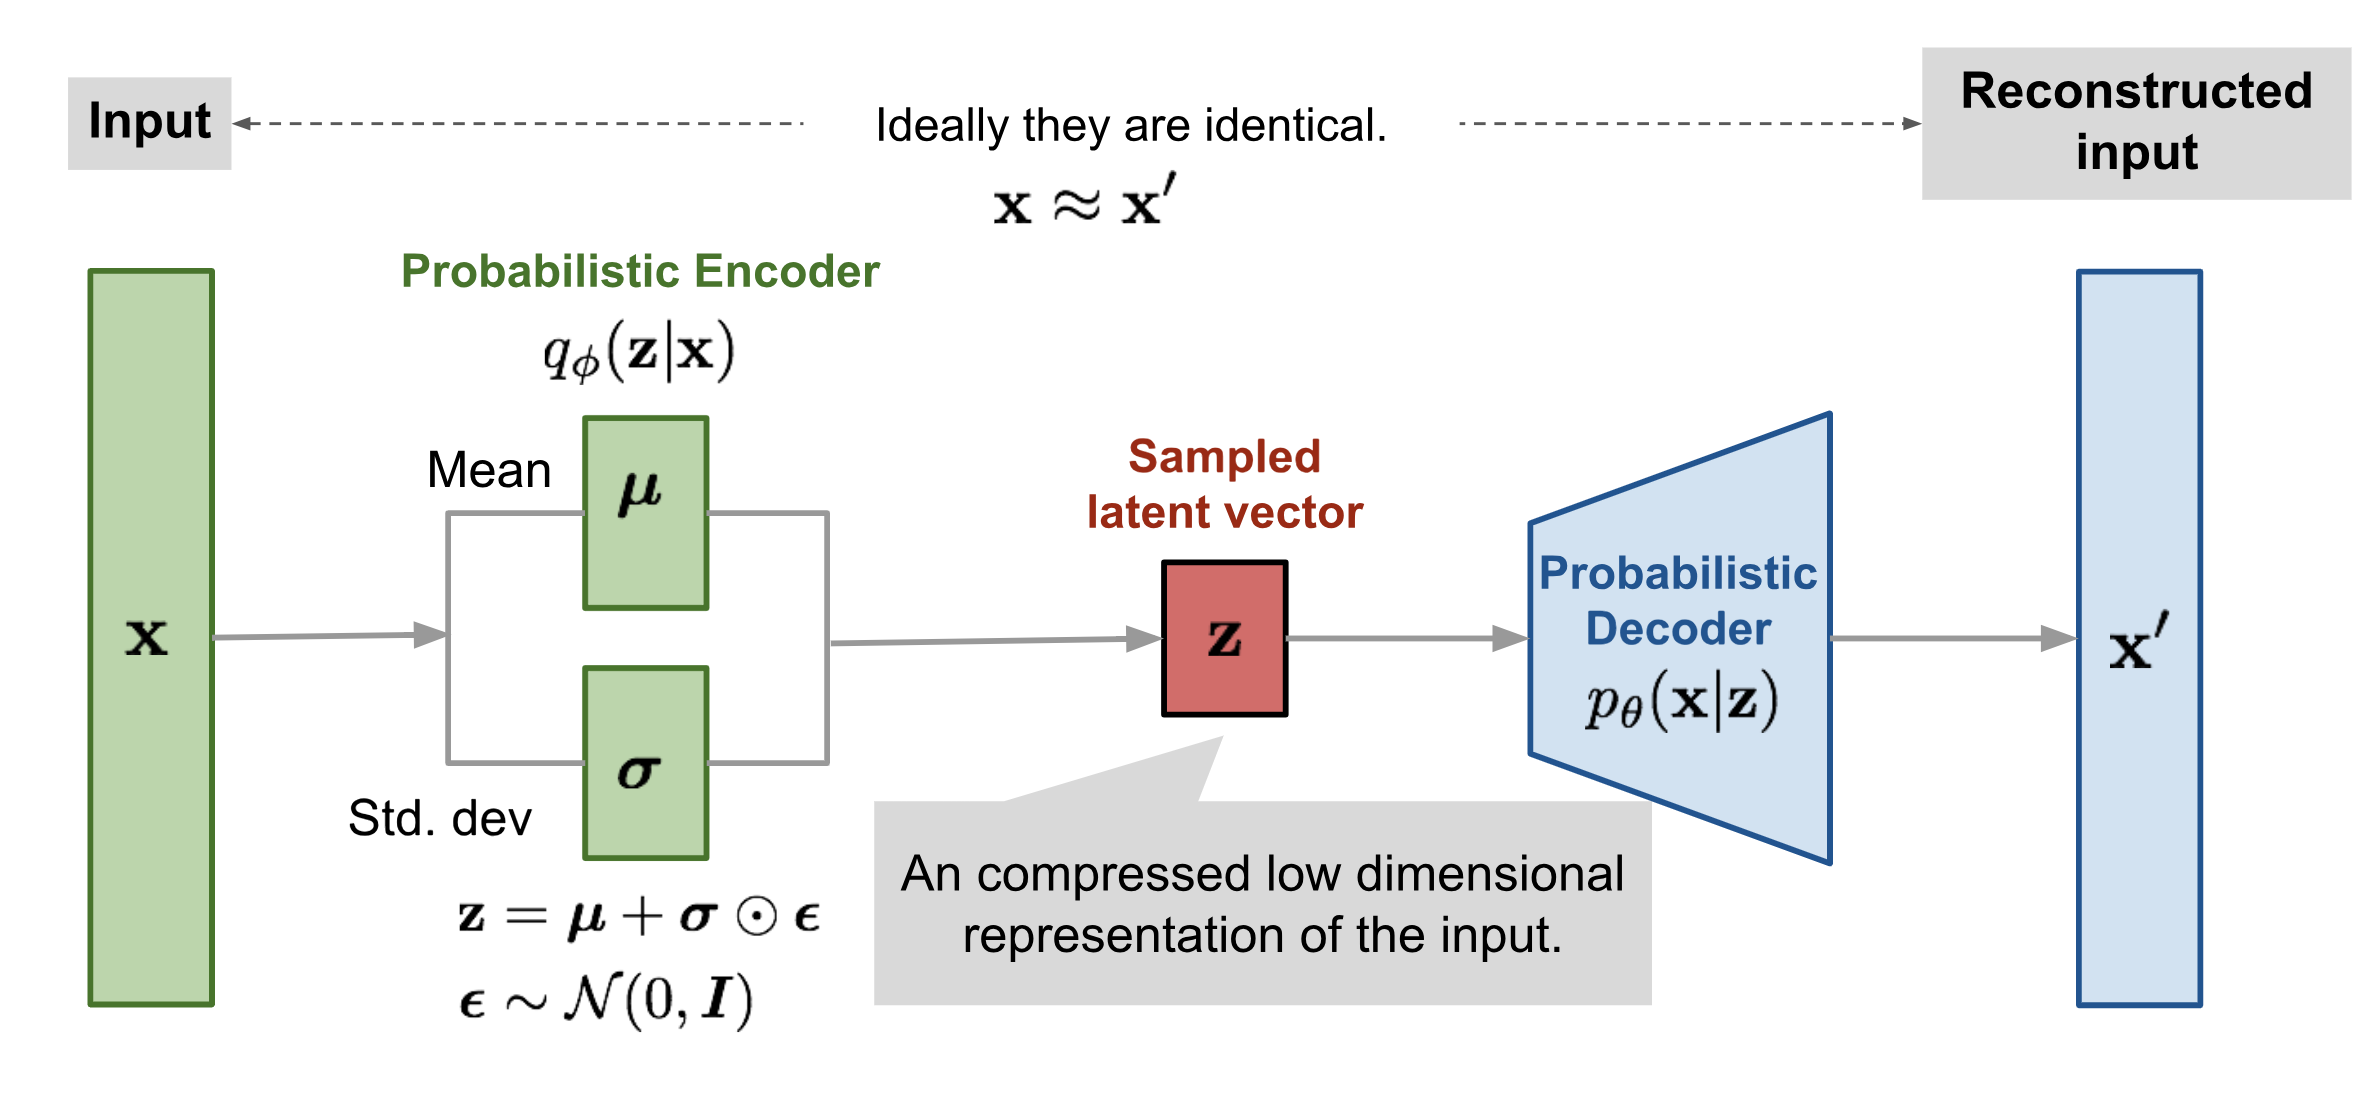
\includegraphics[width=\linewidth]{figs/vae-gaussian.png}
	\end{figure}
	
	\myfootnotewithlink{https://lilianweng.github.io/lil-log/2018/08/12/from-autoencoder-to-beta-vae.html}{image credit: https://lilianweng.github.io/lil-log/2018/08/12/from-autoencoder-to-beta-vae.html}
\end{frame}
%=======
\begin{frame}{Bayesian framework}
	\begin{block}{Posterior distribution}
		\vspace{-0.2cm}
		\[
			p(\btheta | \bX) = \frac{p(\bX | \btheta) p(\btheta)}{p(\bX)} = \frac{p(\bX | \btheta) p(\btheta)}{\int p(\bX | \btheta) p(\btheta) d \btheta} 
		\]
		\vspace{-0.2cm}
	\end{block}
	\begin{block}{Bayesian inference}
		\vspace{-0.3cm}
		\[
			p(\bx | \bX) = \int p(\bx | \btheta) p(\btheta | \bX) d \btheta
		\]
	\end{block}
    \begin{block}{Maximum a posteriori (MAP) estimation}
	    \vspace{-0.3cm}
	    \[
	        \btheta^* = \argmax_{\btheta} \log p(\btheta | \bX) = \argmax_{\btheta} \bigl(\log p(\bX | \btheta) + \log p(\btheta) \bigr)
	    \]
        \vspace{-0.3cm}
    \end{block}
	\begin{block}{MAP inference}
		\vspace{-0.4cm}
		\[
			p(\bx | \bX) = \int p(\bx| \btheta) p(\btheta | \bX ) d \btheta =  \int p(\bx| \btheta) \delta (\btheta - \btheta^* ) d \btheta \approx p(\bx | \btheta^*).
		\]
	\end{block}
\end{frame}
%=======
\begin{frame}{VAE as Bayesian model}
	\begin{block}{Posterior distribution}
		\vspace{-0.2cm}
		\[
			p(\btheta | \bX) = \frac{p(\bX | \btheta) p(\btheta)}{p(\bX)}
		\]
		\vspace{-0.5cm}
	\end{block}
	\begin{block}{ELBO}
		\vspace{-0.5cm}
		\begin{align*}
			 \log p(\btheta | \bX) &= \log p(\bX | \btheta) + \log p(\btheta) - \log p(\bX) \\
			 &= \cL(q, \btheta) + KL(q || p) + \log p(\btheta) - \log p(\bX) \\
			 &\geq \left[ \cL(q, \btheta) + \log p(\btheta) \right] - \log p(\bX) .
		\end{align*}
		\vspace{-0.7cm}
	\end{block}
	\begin{block}{EM-algorithm}
		\begin{itemize}
			\item E-step
				\vspace{-0.2cm}
				\[
					q(\bz) = \argmax_q \mathcal{L} (q, \btheta^*) = \argmin_q KL(q || p) =
				 p(\bz| \bx, \btheta^*);
				\]
				\vspace{-0.5cm}
			\item M-step
				\[
					\btheta^* = \argmax_{\btheta} \left[ \mathcal{L} (q, \btheta) + \log p(\btheta) \right].
				\]
		\end{itemize}
	\end{block}
\end{frame}
%=======
\begin{frame}{VAE limitations}
	\begin{itemize}
		\item Poor variational posterior distribution (inference model encoder)
		\[
		q(\bz | \bx, \bphi) = \mathcal{N}(\bz| \bmu_{\bphi}(\bx), \bsigma^2_{\bphi}(\bx)).
		\]
		\item Poor prior distribution
		\[
		p(\bz) = \mathcal{N}(0, \mathbf{I}).
		\]
		\item Poor probabilistic model (generative model, decoder)
		\[
		p(\bx | \bz, \btheta) = \mathcal{N}(\bx| \bmu_{\btheta}(\bz), \bsigma^2_{\btheta}(\bz)).
		\]
		\item Loose lower bound
		\[
		\log p(\bx | \btheta) - \mathcal{L}(q, \btheta) = (?).
		\]
	\end{itemize}
\end{frame}
%=======
\begin{frame}{Likelihood-based models so far...}
	\begin{minipage}[t]{0.5\columnwidth}
		\begin{block}{Autoregressive models}
			\vspace{-0.5cm}
			\[
			p(\bx|\btheta) = \prod_{i=1}^m p(x_i | \bx_{1:i - 1}, \btheta)
			\]
			\vspace{-0.2cm}
			\begin{itemize}
				\item tractable likelihood, 
				\item no inferred latent factors.
			\end{itemize}
		\end{block}
	\end{minipage}%
	\begin{minipage}[t]{0.5\columnwidth}
		\begin{block}{Latent variable models}
			\[
			p(\bx| \btheta) = \int p(\bx, \bz | \btheta) d \bz
			\]
			\begin{itemize}
				\item latent feature representation, 
				\item intractable likelihood.
			\end{itemize}
		\end{block}
	\end{minipage}
	
	\vspace{1cm } 
	How to build model with latent variables and tractable likelihood?
\end{frame}
%=======
\begin{frame}{Flows intuition}
	Let $\xi$ be a random variable with density $p(\xi)$. Then
	\[
	\eta = F(\xi) = \int_{-\infty}^\xi p(t)dt \sim U[0, 1].
	\]
	\[
		P(\eta < y) = P(F(\xi) < y) = P(\xi < F^{-1}(y)) = F(F^{-1}(y)) = y
	\]
	Hence
	\[
	\eta \sim U[0, 1]; \quad \xi = F^{-1}(\eta) \quad \Rightarrow \quad \xi \sim p(\xi).
	\]
	\begin{figure}
		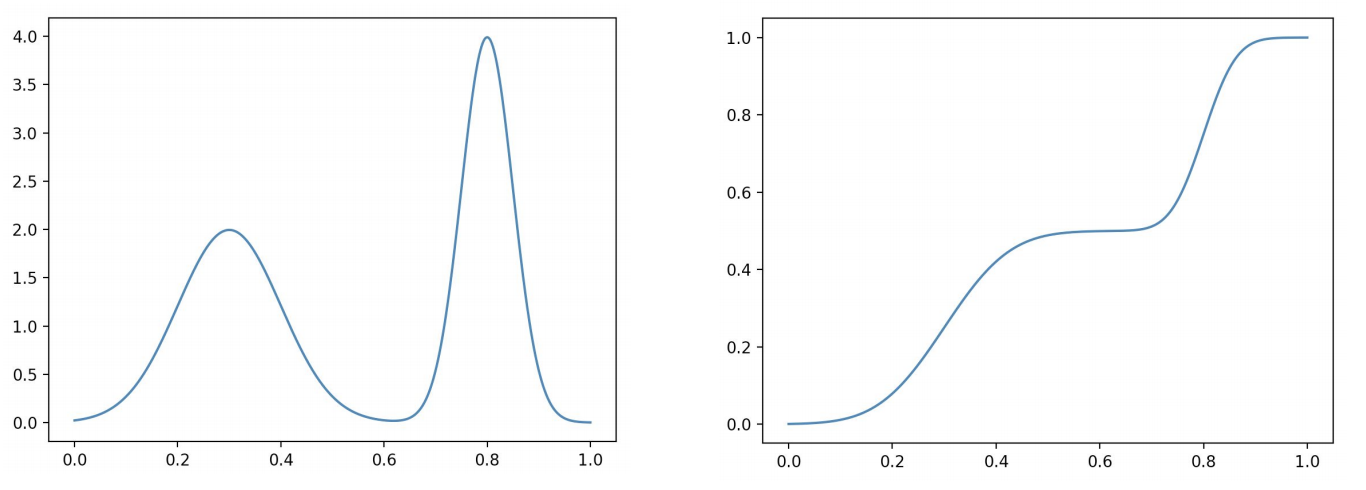
\includegraphics[width=\linewidth]{figs/flows_1d}
	\end{figure}
	\myfootnotewithlink{https://sites.google.com/view/berkeley-cs294-158-sp19/home}{image credit: https://sites.google.com/view/berkeley-cs294-158-sp19/home}
	
\end{frame}
%=======
\begin{frame}{Flows intuition}
	\begin{itemize}
		\item Let $z \sim p(z)$ is a random variable with base distribution $p(z) = U[0, 1]$. 
		\item Let $x \sim p(x)$ is a random variable with complex distribution $p(x)$ and cdf $F(x)$. 
		\item Then noise variable $z$ can be transformed to $x$ using inverse cdf~$F^{-1}$ ($x = F^{-1}(z)$).
	\end{itemize}
	How to transform random variable $z$  which has a distribution different from uniform to $x$?
		\begin{itemize}
			\item Let $z \sim p(z)$ is a random variable with base distribution $p(z)$ and cdf $G(z)$.
			\item Then $z_0 = G(z)$ has base distribution $p(z_0) = U[0, 1]$.
			\item Let $x \sim p(x)$ is a random variable with complex distribution $p(x)$ and cdf $F(x)$. 
			\item Then noise variable $z$ can be transformed to $x$ using cdf $G$ and inverse cdf~$F^{-1}$ ($x = F^{-1}(z_0) = F^{-1}(G(z))$).
		\end{itemize}
\end{frame}
%=======
\begin{frame}{Change of variables}
	\begin{block}{Theorem}
		\begin{itemize}
			\item $\bx$ is a random variable with density function $p(\bx)$;
			\item $f: \mathbb{R}^m \rightarrow \mathbb{R}^m$ is a differentiable, invertible function (diffeomorphism);
			\item $\bz = f(\bx)$, $\bx = f^{-1}(\bz) = g(\bz)$ (here $g = f^{-1}$).
		\end{itemize}
		Then
		\vspace{-0.3cm}
		\begin{align*}
			p(\bx) &= p(\bz) \left|\det \left(  \frac{\partial \bz}{\partial \bx} \right) \right| = p(f(\bx)) \left|\det \left(  \frac{\partial f(\bx)}{\partial \bx} \right) \right| \\
			p(\bz) &= p(\bx) \left|\det \left(  \frac{\partial \bx}{\partial \bz} \right) \right| = p(g(\bz)) \left|\det \left(  \frac{\partial g(\bz)}{\partial \bz} \right) \right|.
		\end{align*}
	\end{block}
		\begin{itemize}
			\item $\bx$ and $\bz$ have the same dimensionality (lies in $\bbR^m$);
			\item $ \left|\det \left(  \frac{\partial f(\bx)}{\partial \bx} \right)\right| = \left|\det \left(  \frac{\partial g^{-1}(\bx)}{\partial \bx} \right)\right| = \left|\det \left(  \frac{\partial g(\bz)}{\partial \bz} \right)\right|^{-1}$;
			\item $f(\bx, \btheta)$ could be parametric function.
		\end{itemize}
\end{frame}
%=======
\begin{frame}{Fitting flows}
	\begin{block}{MLE problem}
		\vspace{-0.3cm}
		\[
		\btheta^* = \argmax_{\btheta} p(\bX | \btheta) = \argmax_{\btheta} \prod_{i=1}^n p(\bx_i | \btheta) = \argmax_{\btheta} \sum_{i=1}^n \log p(\bx_i | \btheta).
		\]
		\vspace{-0.3cm}
	\end{block}
	\begin{block}{Challenge}
		$p(\bx | \btheta)$ can be intractable.
	\end{block}
	\begin{block}{Fitting flow to solve MLE}
		\[
		p(\bx|\btheta) = p(\bz) \left|\det \left(  \frac{\partial \bz}{\partial \bx} \right) \right|  = p(f(\bx, \btheta)) \left|\det \left( \frac{\partial f(\bx, \btheta)}{\partial \bx} \right) \right|
		\]
		\[
			\log p(\bx|\btheta) = \log p(f(\bx, \btheta)) + \log  \left|\det \left( \frac{\partial f(\bx, \btheta)}{\partial \bx} \right) \right|
		\]
	\end{block}
\end{frame}
%=======
\begin{frame}{Flows}
	\begin{figure}
		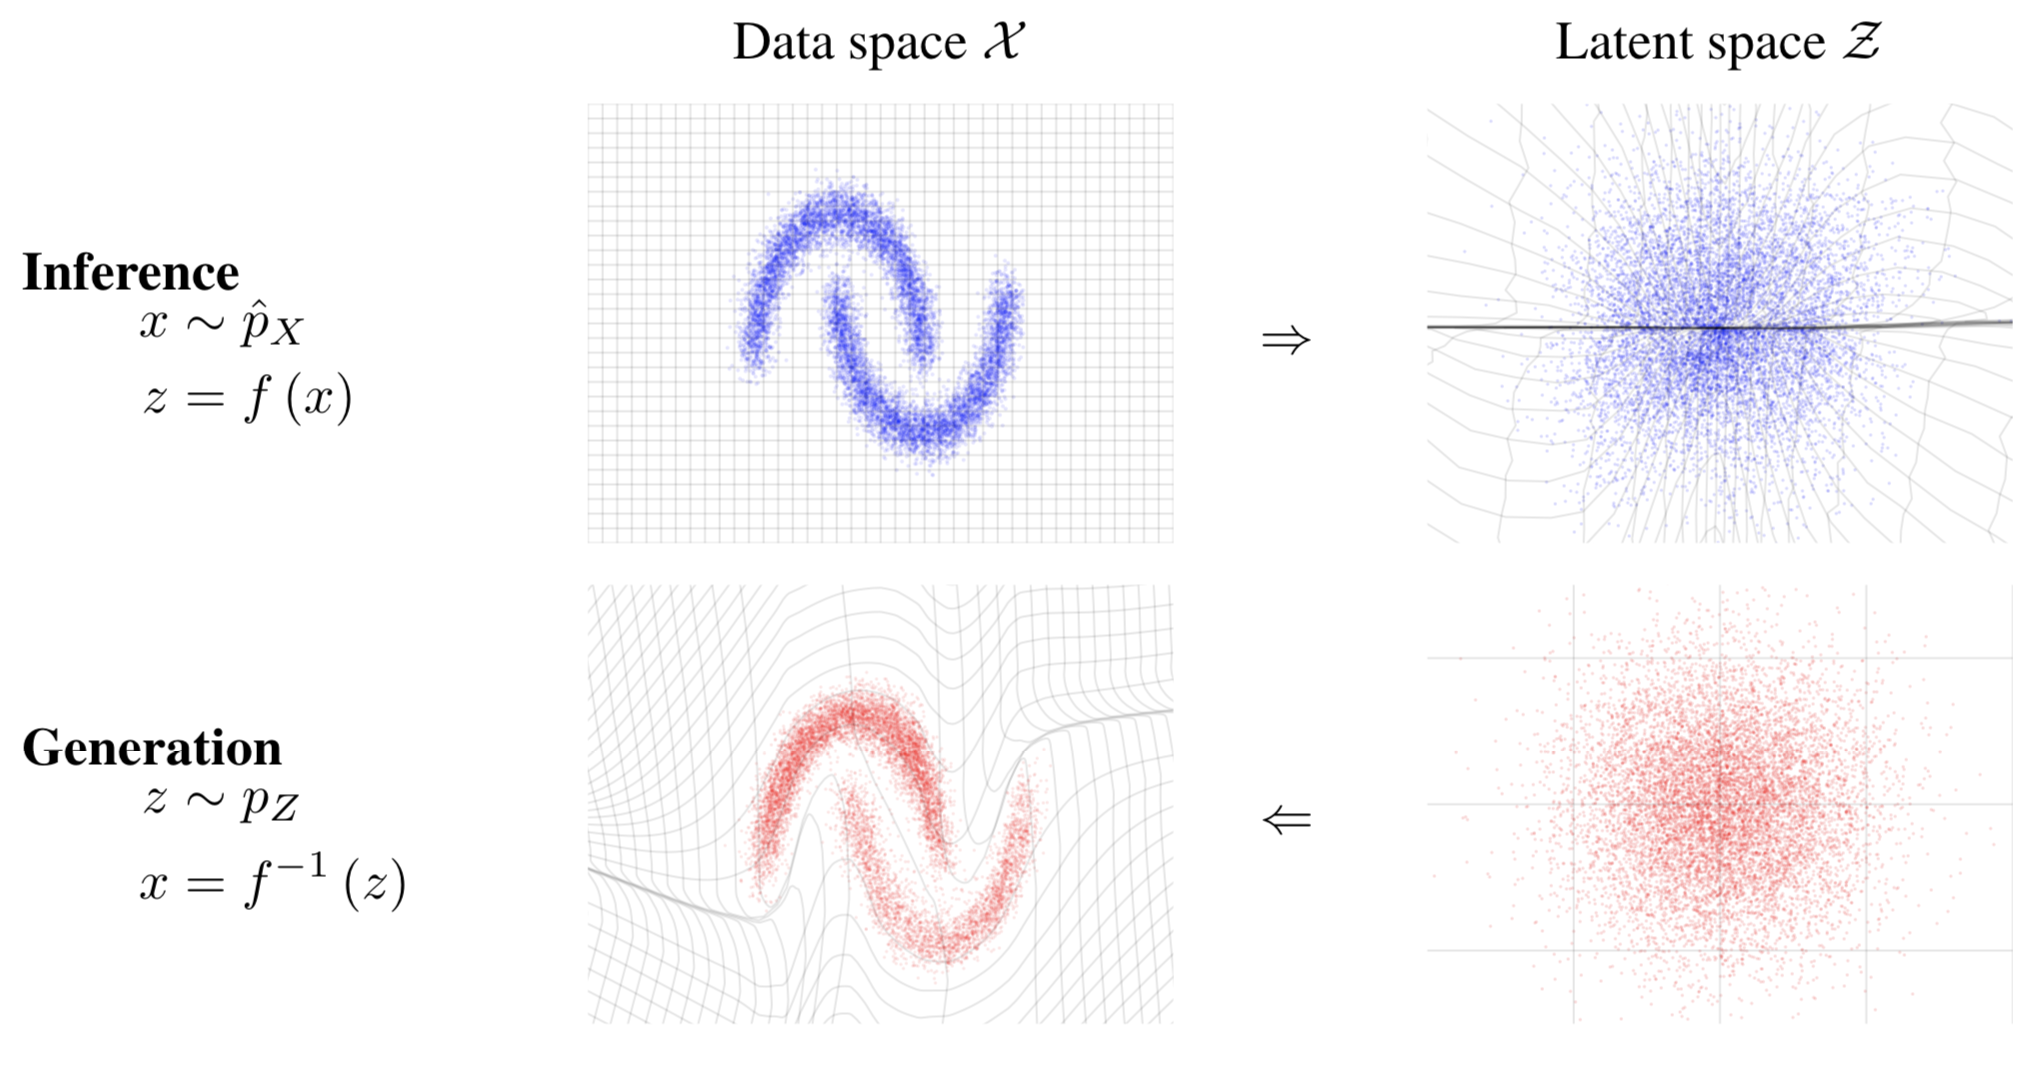
\includegraphics[width=0.7\linewidth]{figs/flows_how2.png}
	\end{figure}
	\vspace{-0.3cm}
	\begin{block}{Computational requirement}
		\begin{itemize}	
			\item Evaluating model density $p(\bx | \btheta)$ requires computing the transformation $\bz = f(\bx,  \btheta)$ and its Jacobian determinant $\left|\det \left( \frac{\partial f(\bx, \btheta)}{\partial \bx} \right) \right|$,
			and evaluating the density $p(\bz)$.
			\item Sampling $\bx$ from the model requires the ability to sample from $p(\bz)$ and to compute the transformation $\bx = g(\bz, \btheta) = f^{-1}(\bz, \btheta)$. 
		\end{itemize}
	\end{block}
	\myfootnotewithlink{https://arxiv.org/abs/1605.08803}{Dinh L., Sohl-Dickstein J., Bengio S. Density estimation using Real NVP, 2016} 
\end{frame}
%=======
\begin{frame}{Forward KL vs Reverse KL}
	Fix probabilistic model $p(\bx | \btheta)$~-- the set of parameterized distributions . \\
	Instead of searching true $\pi(\bx)$ over all probability distributions, learn function approximation $p(\bx | \btheta) \approx \pi(\bx)$.
	\begin{block}{Forward KL}
		\vspace{-0.2cm}
		\[
			KL(\pi || p) = \int \pi (\bx) \log \frac{\pi(\bx)}{p(\bx | \btheta)} d \bx \rightarrow \min_{\btheta}
		\]
	\end{block}
	\begin{block}{Reverse KL}
		\vspace{-0.2cm}
		\[
			KL(p || \pi) = \int p (\bx| \btheta) \log \frac{p(\bx| \btheta)}{\pi(\bx)} d \bx \rightarrow \min_{\btheta}
		\]
	\end{block}
	\begin{itemize}
		\item What is the difference between these two formulations?
		\item What do we get in these two cases if $p(\bx | \btheta)$ is a flow model?
	\end{itemize}
\end{frame}
%=======
\begin{frame}{Forward KL vs Reverse KL}
	\begin{block}{Forward KL}
		    \vspace{-0.5cm}
		\begin{align*}
			KL(\pi || p) &= \int \pi (\bx) \log \frac{\pi(\bx)}{p(\bx | \btheta)} d \bx \\
			&= \int \pi (\bx) \log \pi(\bx) d \bx - \int \pi (\bx) \log p(\bx | \btheta) d \bx \\
			&= - \bbE_{\pi(\bx)} \log p(\bx | \btheta) + \text{const} \rightarrow \min_{\btheta}
		\end{align*}
		\vspace{-0.5cm}
	\end{block}
	\begin{block}{Monte-Carlo estimation}
		\vspace{-0.5cm}
		\[
			KL(\pi || p) = - \bbE_{\pi(\bx)} \log p(\bx | \btheta) + \text{const} \approx - \frac{1}{n} \sum_{i=1}^n \log p(\bx_i | \btheta) \rightarrow \min_{\btheta}.
		\]
		\vspace{-0.5cm}
	\end{block}
	    \begin{block}{MLE problem}
	    \vspace{-0.5cm}
	    \[
	        \btheta^* = \argmax_{\btheta} p(\bX | \btheta) = \argmax_{\btheta} \prod_{i=1}^n p(\bx_i | \btheta) = \argmax_{\btheta} \sum_{i=1}^n \log p(\bx_i | \btheta).
	    \]
	    \vspace{-0.1cm}
	    \end{block}
\end{frame}
%=======
\begin{frame}{Forward KL vs Reverse KL}
	\begin{block}{Forward KL}
	    \vspace{-0.3cm}
		\[
			\btheta^* = \argmax_{\btheta} \frac{1}{n} \sum_{i=1}^n \log p(\bx_i | \btheta) \approx  \argmin_{\btheta} KL(\pi || p)
		\]
		Maximum likelihood estimation is equivalent to minimization of the Monte-Carlo estimation of forward KL.
	\end{block}
	\begin{block}{Forward KL for flow model}
	    \vspace{-0.3cm}
		\[
			\log p(\bx|\btheta) = \log p(f(\bx, \btheta)) + \log  \left|\det \left( \frac{\partial f(\bx, \btheta)}{\partial \bx} \right) \right|
		\]
		\begin{itemize}
		\item We need to be able to compute $f(\bx, \btheta)$ and its Jacobian.
		\item We need to be able to compute the density $p(\bz)$.
		\item We don’t need to think about computing the function $g(\bz, \btheta) = f^{-1}(\bz, \btheta)$ until we want to sample from the flow.
		\end{itemize}
	\end{block}
\end{frame}
%=======
\begin{frame}{Forward KL vs Reverse KL}
	\begin{block}{Reverse KL}
	  	\vspace{-0.5cm}
			\begin{align*}
				KL(p || \pi) &= \int p(\bx | \btheta) \log \frac{p(\bx | \btheta)}{\pi(\bx)} d \bx \\
				&= \bbE_{p(\bx | \btheta)} \left[\log p(\bx | \btheta) - \log \pi(\bx)\right] \rightarrow \min_{\btheta}
			\end{align*}
		\vspace{-0.7cm}
	\end{block}
	\begin{block}{Reverse KL for flow model}
  		\vspace{-0.3cm}
		\[
			\log p(\bz) = \log p(\bx | \btheta) + \log \left|\det \left( \frac{\partial g(\bz, \btheta)}{\partial \bz} \right) \right|
		\]
		\[
			KL(p || \pi)  = \bbE_{p(\bz)} \left[  \log p(\bz) - \log \left|\det \left( \frac{\partial g(\bz, \btheta)}{\partial \bz} \right) \right| - \log \pi(g(\bz, \btheta)) \right]
		\]
		\begin{itemize}
		\item We need to be able to compute $g(\bz, \btheta)$ and its Jacobian.
		\item We need to be able to sample from the density $p(\bz)$ (do not need to evaluate it).
		\item We don’t need to think about computing the function $f(\bx, \btheta)$.
		\end{itemize}
	\end{block}
\end{frame}
%=======
\begin{frame}{Composition of flows}
	\begin{block}{Theorem}
		Diffeomorphisms are \textbf{composable} (If $f_1, f_2$ satisfy conditions of the change of variable theorem (differentiable and invertible), then $\bz = f(\bx) = f_2 \circ f_1(\bx)$ also satisfies it).
	\end{block}
	\begin{multline*}
		p(\bx) = p(\bz) \left|\det \left(  \frac{\partial \bz}{\partial \bx} \right) \right| = p(f(\bx)) \left|\det \left(  \frac{\partial f(\bx)}{\partial \bx} \right) \right| = \\
		= p(f(\bx)) \left|\det \left(\frac{\partial f_2 \circ f_1(\bx)}{\partial \bx} \right) \right| =
		p(f(\bx)) \left|\det \left(\frac{\partial \textbf{f}_2}{\partial \textbf{f}_1} \cdot \frac{\partial \textbf{f}_1}{\partial \bx} \right) \right| = \\
		= p(f(\bx))  \left|\det \left(\frac{\partial \textbf{f}_2}{\partial \textbf{f}_1} \right) \right| \cdot \left| \det \left( \frac{\partial \textbf{f}_1}{\partial \bx} \right) \right|
	\end{multline*}

	What will we get in the case $\bz = f(\bx) = f_n \circ \dots \circ f_1(\bx)$?
\end{frame}
%=======
\begin{frame}{Flows}
	\vspace{-0.3cm}
	\[
		\log p(\bx|\btheta) = \log p(f(\bx, \btheta)) + \log \left|\det \left( \frac{\partial f(\bx, \btheta)}{\partial \bx} \right) \right|
	\]
	\vspace{-0.3cm}
	\begin{block}{Definition}
		Normalizing flow is a \textit{differentiable, invertible} mapping from data $\bx$ to the noise $\bz$. 
	\end{block}
	\begin{itemize}
		\item "Normalizing" means that the inverse flow takes samples from $p(\bx)$ and normalizes them into samples from density $p(\bz)$.
		\item "Flow" refers to the trajectory followed by samples from $p(\bz)$ as they are transformed by the sequence of transformations
		\[
		\bz = f_K \circ \dots \circ f_1(\bx); \quad \bx = f_1^{-1} \circ \dots \circ f_K^{-1} (\bz) = g_1 \circ \dots \circ g_K(\bz) 
		\] 
		\begin{multline*}
			p(\bx) = p(f_K \circ \dots \circ f_1(\bx)) \left|\det \left(\frac{\partial f_K \circ \dots \circ f_1(\bx)}{\partial \bx} \right) \right| = \\
			= p(f_K \circ \dots \circ f_1(\bx)) \prod_{k=1}^K \left|\det \left(\frac{\partial \mathbf{f}_k}{\partial \mathbf{f}_{k-1}} \right) \right|.
		\end{multline*}
	\end{itemize}
\end{frame}
%=======
\begin{frame}{Flows}
	\begin{block}{Example of a 4-step flow}
	\vspace{-0.2cm}
	\begin{figure}
			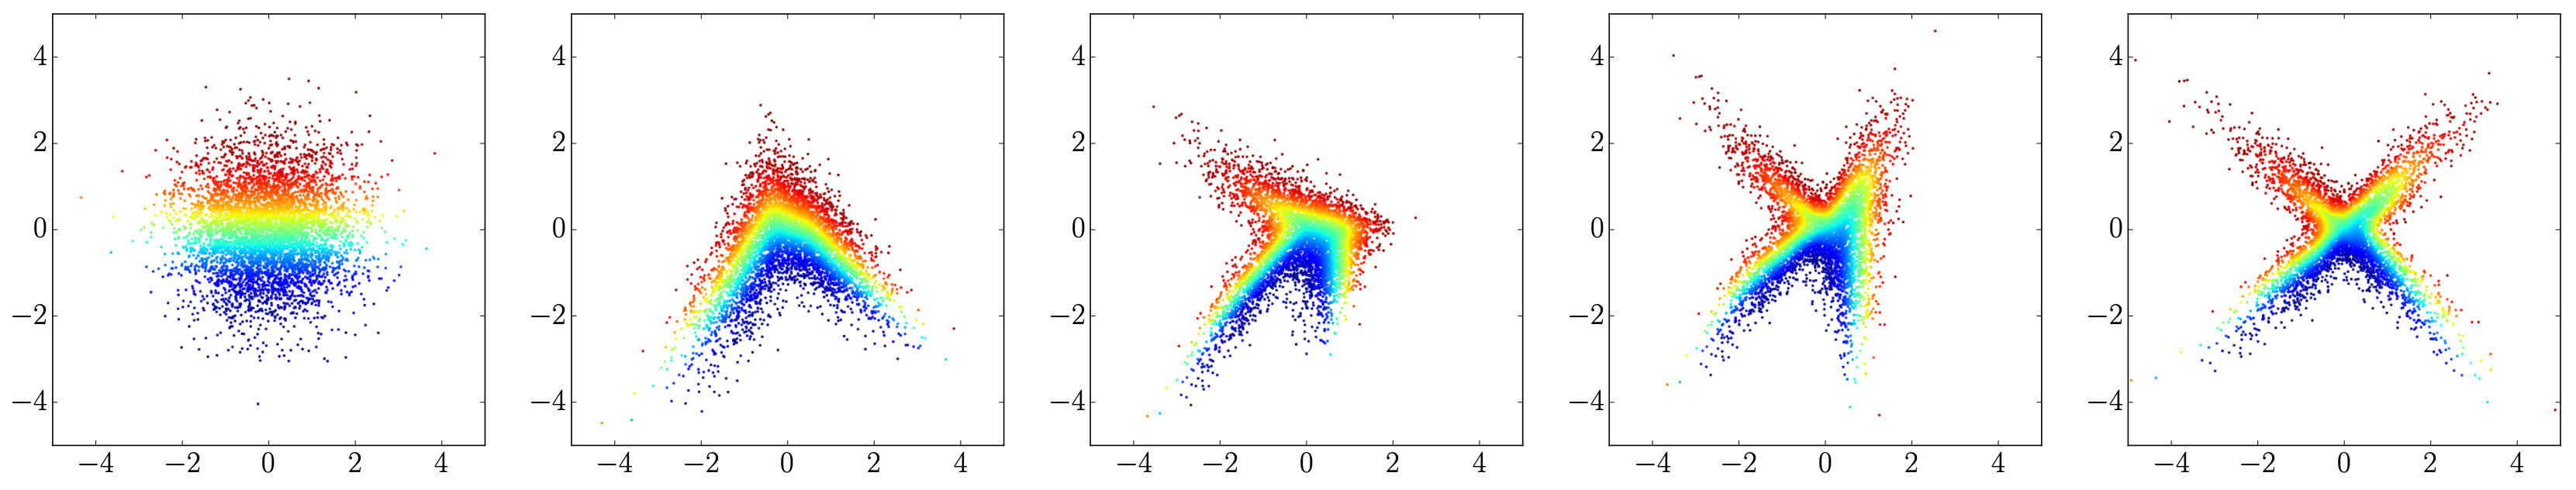
\includegraphics[width=\linewidth]{figs/flow_4_steps_example.png}
	\end{figure}
	\end{block}
	\vspace{-0.3cm}
	\begin{block}{Flow likelihood}
		\vspace{-0.3cm}
		\[
		\log p(\bx|\btheta) = \log p(f(\bx, \btheta)) + \log \left|\det \left( \frac{\partial f(\bx, \btheta)}{\partial \bx} \right) \right|
		\]
		\vspace{-0.3cm}
	\end{block}
	What is the complexity of the determinant computation?
	\begin{block}{What we want}
		\begin{itemize}
			\item Efficient computation of Jacobian $\frac{\partial f(\bx, \btheta)}{\partial \bx}$;
			\item Efficient sampling from the base distribution $p(\bz)$;
			\item Efficient inversion of $f(\bx, \btheta)$.
		\end{itemize}
		
	\end{block}
		\myfootnotewithlink{https://arxiv.org/abs/1912.02762}{Papamakarios G. et al. Normalizing flows for probabilistic modeling and inference, 2019} 
\end{frame}
%=======
\begin{frame}{Summary}
	\begin{itemize}
	\item The reparametrization trick gets unbiased gradients w.r.t to a variational posterior distribution.
	\vfill
	\item The VAE model is an LVM with two neural network: for stochastic encoder $q(\bz | \bx, \bphi)$ and for stochastic decoder $p(\bx | \bz, \btheta)$.
	\vfill
	\item VAE is not a "true" bayesian model since parameters $\btheta$ do not have a prior distribution.
	\vfill
	\item Standart VAE has several limitations that we will address later in the course.
	\vfill
	\item Forward KL minimization is equivalent to MLE. Reverse KL is used in variational inference.
	\vfill
	\item Flow models transform a simple base distribution to a complex one via a sequence of invertible transformations.
	\vfill
	\item Flow models have a tractable likelihood that is given by the change of variable theorem.
	\end{itemize}
\end{frame}
\end{document} 